\section{K Means Clustering} 

  We will start off with conceptually the simplest form of clustering, although not the earliest developed. K-means was published at 1967 in \cite{1967macqueen}, but has been discovered in the 1950s. The general idea is that given an integer $K$, we want to find $K$ \textit{centroids} that provide a good approximation of where the clusters are in the data. We can quantify what a good approximation is by taking the distance from a sample to its closest cluster centroid.

  \begin{definition}[K Means Clustering]
    A \textbf{K-means clustering} model is an parameteric unsupervised model with parameters $\{\mu_1, \ldots, \mu_K\}$ representing clusters that each sample belongs to. The cluster that sample $x$ belongs to is 
    \begin{equation}
      \mathrm{cluster}(x) = \argmin_{\mu_k} d(x, \mu_k)
    \end{equation}
    Usually, we let $d$ be the $L^2$ metric in Euclidean space. 
  \end{definition}

  \begin{theorem}[Risk]
    The expected risk of $K$-means is 
    \begin{equation}
      R(\mu_1, \ldots, \mu_K) = \mathbb{E}_x \left[ \min_{k \in [K]} \| x - \mu_k \|^2 \right] = \int \min_{k \in [K]} \| x - \mu_k \|^2 \,dx
    \end{equation} 
    and our empirical risk for a dataset $\mathcal{D} = \{x^{(i)}\}_{i=1}^n$ is therefore 
    \begin{equation}
      \hat{R}(\mu_1, \ldots, \mu_K) = \frac{1}{n} \sum_{i=1}^n \min_{k \in [K]} \| x^{(i)} - \mu_k \|^2
    \end{equation} 
  \end{theorem} 

\subsection{NP-Hardness}

  So we have reduced this model into an optimization problem of the appropriate risk. Let's try and analyze how hard this is. 

  \begin{theorem}
    For a fixed dimension $d$ and number of clusters $K$, we can minimize the empirical risk in $O(n^{dk + 1})$. 
  \end{theorem} 

  \begin{theorem}
    For any fixed $d$ (even $d = 2$), minimizing the empirical risk over all $K$ is NP-hard. 
  \end{theorem}

  Therefore, we must rely on approximate algorithms. 

\subsection{Lloyd's Algorithm}

  Great, we have an almost-everywhere differentiable function, which can be solved with gradient methods like SGD or coordinate descent. The problem is that this is not necessarily convex. 

  \begin{theorem}[Convergence of Coordinate Descent]
    
  \end{theorem}
  
  Now that convergence is guaranteed, constructing the algorithm is straightforward. In fact, it is precisely coordinate descent!  

  \begin{algo}[Lloyd's Algorithm]
    The algorithm intuitively initializes the centroids randomly, and then moves them to the center of each cluster through the two stage process: 
    \begin{enumerate}
      \item Assigning each training sample $x^{(i)}$ to the closest cluster centroid $\mu_k$. 
      \item Move each training cluster centroid $\mu_k$ to the mean of the points assigned to it. 
    \end{enumerate}
    \begin{algorithm}[H]
    \caption{K-Means Clustering}
    \label{alg:kmeans}
    \begin{algorithmic}[1]
      \Procedure{KMeans}{$\mathbf{X}, K$}
          
      \Require{Dataset $\mathbf{X} = \{x^{(1)}, x^{(2)}, \ldots, x^{(n)}\}$ where $x^{(i)} \in \mathbb{R}^d$, number of clusters $K$}
      \Ensure{Cluster centroids $\mu_1, \mu_2, \ldots, \mu_K$ and cluster assignments $c^{(1)}, c^{(2)}, \ldots, c^{(n)}$}
      
      % Initialization
      \State Initialize cluster centroids $\mu_1, \mu_2, \ldots, \mu_K \in \mathbb{R}^d$ randomly
      
      % Main loop
      \Repeat
        % Assignment step
        \For{$i \gets 1$ to $n$}
          \State $c^{(i)} \gets \arg\min_j ||x^{(i)} - \mu_j||^2$
        \EndFor
        
        % Update step
        \For{$j \gets 1$ to $K$}
          \State $\mu_j \gets \frac{\sum_{i=1}^n \mathbf{1}\{c^{(i)} = k\} x^{(i)}}{\sum_{i=1}^n \mathbf{1}\{c^{(i)} = k\}}$
        \EndFor
      \Until{convergence}
      
      \State \Return $\mu_1, \mu_2, \ldots, \mu_K, c^{(1)}, c^{(2)}, \ldots, c^{(n)}$
      \EndProcedure
    \end{algorithmic}
    \end{algorithm}
  \end{algo} 

  \begin{example}[K-Means Walkthrough]
    Let us walk through how the centroids evolve visually on a toy dataset. 

    \begin{figure}[H]
      \centering
      \begin{subfigure}[b]{0.48\textwidth}
        \centering
        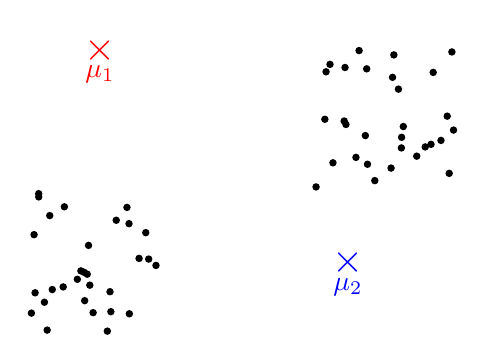
\begin{tikzpicture}[scale=0.9]
          \pgfmathsetseed{42}
          \foreach \i in {1,...,30} { 
            \pgfmathsetmacro{\x}{-2 + 2*rnd }
            \pgfmathsetmacro{\y}{-1 + 2*rnd}
            \fill[black] (\x,\y) circle (1.5pt);
          }

          \foreach \i in {1,...,30} {
            \pgfmathsetmacro{\x}{2 + 2*rnd}
            \pgfmathsetmacro{\y}{1 + 2*rnd}
            \fill[black] (\x,\y) circle (1.5pt);
          }

          % Left centroid
          \node[red, font=\Large] at (-1,3) {$\times$};
          \node[red, below=2pt] at (-1,3) {$\mu_1$};

          % Right centroid
          \node[blue, font=\Large] at (2.5,0) {$\times$};
          \node[blue, below=2pt] at (2.5,0) {$\mu_2$};
        \end{tikzpicture}
        \caption{We initialize the centroids $\mu_1, \mu_2$ randomly.}
      \end{subfigure}
      \hfill 
      \begin{subfigure}[b]{0.48\textwidth}
        \centering
        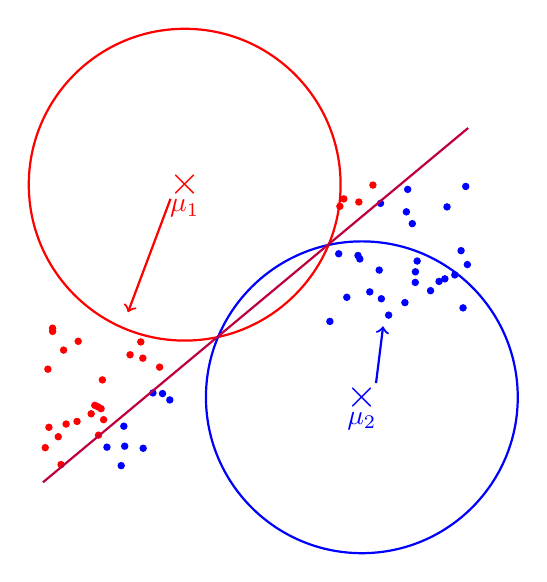
\begin{tikzpicture}[scale=0.9]
          \pgfmathsetseed{42}
          \foreach \i in {1,...,30} { 
            \pgfmathsetmacro{\x}{-2 + 2*rnd }
            \pgfmathsetmacro{\y}{-1 + 2*rnd}
            % Calculate if point is above or below the purple line y = 0.833x + 0.467
            \pgfmathsetmacro{\liney}{0.833*\x + 0.467}
            \pgfmathsetmacro{\isabove}{\y > \liney ? 1 : 0}
            \ifnum\isabove=1
              \fill[red] (\x,\y) circle (1.5pt);
            \else
              \fill[blue] (\x,\y) circle (1.5pt);
            \fi
          }
          \foreach \i in {1,...,30} {
            \pgfmathsetmacro{\x}{2 + 2*rnd}
            \pgfmathsetmacro{\y}{1 + 2*rnd}
            % Calculate if point is above or below the purple line y = 0.833x + 0.467
            \pgfmathsetmacro{\liney}{0.833*\x + 0.467}
            \pgfmathsetmacro{\isabove}{\y > \liney ? 1 : 0}
            \ifnum\isabove=1
              \fill[red] (\x,\y) circle (1.5pt);
            \else
              \fill[blue] (\x,\y) circle (1.5pt);
            \fi
          }
          % Left centroid
          \node[red, font=\Large] at (0,3) {$\times$};
          \node[red, below=2pt] at (0,3) {$\mu_1$};
          \draw[red, thick] (0,3) circle (2.2cm);  % Red circle around μ₁
          
          % Right centroid
          \node[blue, font=\Large] at (2.5,0) {$\times$};
          \node[blue, below=2pt] at (2.5,0) {$\mu_2$};
          \draw[blue, thick] (2.5,0) circle (2.2cm);  % Blue circle around μ₂ 
          \draw[purple, thick] (-2, -1.2) -- (4, 3.8);
          \draw[red, thick, ->] (-0.2, 2.8) -- (-0.8, 1.2);
          \draw[blue, thick, ->] (2.7, 0.2) -- (2.8, 1);
        \end{tikzpicture}
        \caption{We classify all points that are in clusters $1$ and $2$. }
      \end{subfigure}

      \begin{subfigure}[b]{0.48\textwidth}
        \centering
        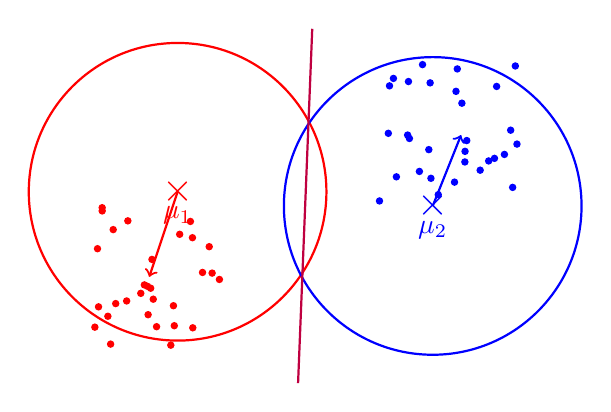
\begin{tikzpicture}[scale=0.9]
          \pgfmathsetseed{42}
          \foreach \i in {1,...,30} { 
            \pgfmathsetmacro{\x}{-2 + 2*rnd }
            \pgfmathsetmacro{\y}{-1 + 2*rnd}
              \fill[red] (\x,\y) circle (1.5pt);
          }
          \foreach \i in {1,...,30} {
            \pgfmathsetmacro{\x}{2 + 2*rnd}
            \pgfmathsetmacro{\y}{1 + 2*rnd} 
            \fill[blue] (\x,\y) circle (1.5pt);
          }
          % Left centroid (moved to arrow head)
          \node[red, font=\Large] at (-0.8,1.2) {$\times$};
          \node[red, below=2pt] at (-0.8,1.2) {$\mu_1$};
          \draw[red, thick] (-0.8,1.2) circle (2.1cm);  % Red circle around μ₁
          
          % Right centroid (moved to arrow head)
          \node[blue, font=\Large] at (2.8,1) {$\times$};
          \node[blue, below=2pt] at (2.8,1) {$\mu_2$};
          \draw[blue, thick] (2.8,1) circle (2.1cm);  % Blue circle around μ₂ 
          
          % New decision boundary line (perpendicular bisector of the line connecting the centroids)
          \draw[purple, thick] (1.1, 3.5) -- (0.9, -1.5);
          \draw[red, thick, ->] (-0.8, 1.2) -- (-1.2, -0);
          \draw[blue, thick, ->] (2.8, 1) -- (3.2, 2);
        \end{tikzpicture}
        \caption{We update the centroids and classify again.}
      \end{subfigure}
      \hfill 
      \begin{subfigure}[b]{0.48\textwidth}
        \centering
        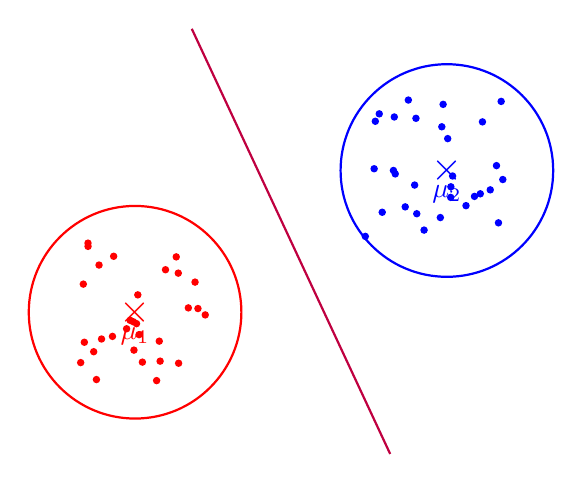
\begin{tikzpicture}[scale=0.9]
          \pgfmathsetseed{42}
          \foreach \i in {1,...,30} { 
            \pgfmathsetmacro{\x}{-2 + 2*rnd }
            \pgfmathsetmacro{\y}{-1 + 2*rnd}
              \fill[red] (\x,\y) circle (1.5pt);
          }
          \foreach \i in {1,...,30} {
            \pgfmathsetmacro{\x}{2 + 2*rnd}
            \pgfmathsetmacro{\y}{1 + 2*rnd} 
            \fill[blue] (\x,\y) circle (1.5pt);
          }
          % Left centroid (moved to arrow head)
          \node[red, font=\Large] at (-1.2, -0) {$\times$};
          \node[red, below=2pt] at (-1.2, -0) {$\mu_1$};
          \draw[red, thick] (-1.2, -0) circle (1.5cm);  % Red circle around μ₁
          
          % Right centroid (moved to arrow head)
          \node[blue, font=\Large] at (3.2, 2) {$\times$};
          \node[blue, below=2pt] at (3.2, 2) {$\mu_2$};
          \draw[blue, thick] (3.2, 2) circle (1.5cm);  % Blue circle around μ₂ 
          
          % New decision boundary line (perpendicular bisector of the line connecting the centroids)
          \draw[purple, thick] (-0.4, 4) -- (2.4, -2);
        \end{tikzpicture}
        \caption{We have convergence.}
      \end{subfigure}
      \caption{A walkthrough for $K$-means clustering for $K = 2$ in $\mathbb{R}^2$.}
      \label{fig:kmeans}
    \end{figure}
  \end{example}

\subsection{Concentration Bounds}

  We can bound the supremum of the expected and exmpirical risk either through the VC dimension or directly with the Rademacher complexity. They both give different bounds, which have advantages and disadvantages. 

  \begin{theorem}
    Let us work over a compact domain. Given that $C^\ast$ is the true risk minimizer and $\hat{C}$ is our empirical risk minimizer, 
    \begin{equation}
      C^\ast = \argmin_{\mu_1, \ldots, \mu_K} R(C), \qquad \hat{C} = \argmin_{\mu_1, \ldots, \mu_K} \hat{R}(C) 
    \end{equation}
    we have 
    \begin{equation}
      \mathbb{E} \left[ | R(C^\ast) - R(\hat{C}) \right] \leq \sqrt{\frac{K (d+1) \log{n}}{n}}
    \end{equation}
  \end{theorem}
  \begin{proof}
    This is proved using VC dimension. 
  \end{proof}

  Let's parse this. So the more clusters you're trying to find---the bigger the $K$---the worse the bound is. More disturbing is the dimension $d$. If $d$ is big, then this is not a very good bound. 

  \begin{theorem}[2008 Gao, Deroit?, Lugacy?]
    Let us work over a compact domain. Given that $C^\ast$ is the true risk minimizer and $\hat{C}$ is our empirical risk minimizer, 
    \begin{equation}
      C^\ast = \argmin_{\mu_1, \ldots, \mu_K} R(C), \qquad \hat{C} = \argmin_{\mu_1, \ldots, \mu_K} \hat{R}(C) 
    \end{equation}
    we have 
    \begin{equation}
      \mathbb{E} \left[ | R(C^\ast) - R(\hat{C}) \right] \leq \frac{K}{n}
    \end{equation}
  \end{theorem}
  \begin{proof}
    This is proved directly using Rademacher complexity. 
  \end{proof}

  The advantage of this is that this bound is dimensionless. This is even true in infinite dimensional Hilbert spaces, which is useful when clustering functions. 

  Now just because the risks are close it does not mean that the clusters are close. You can have two sets of clusters $\{\mu_k\}, \{\mu_k^\prime\}$ that have similar risk but they can be far apart from each other. To control this we need extra assumptions. 

\subsection{Choosing Number of Clusters K}

  Note that the performance of K means really depends on a good choice of $K$. Think about what would have happened if we set $K = 5$ in the walkthrough above. Let's study the impact of changing $K$ a bit more. 

  \begin{theorem}[Expected Risk Decreases as K Increases]
    If $K < K^\prime$, then 
    \begin{equation}
      R(\mu_1, \ldots, \mu_K) \leq R(\mu_1, \ldots, \mu_{K^\prime})
    \end{equation}
  \end{theorem}
  \begin{proof}
    
  \end{proof}



